This chapter reviews previous research into the uses of unintentional EM emanations. Previous studies of unintentional EM emanations mostly focused on security, specifically side channel attacks. We also review electromagnetic compatibility testing and previous work to identify and quantify side channel signals, as well as previous work on the emerging uses of EM emanations outside of side channel attacks. Finally we review traditional approaches to program profiling.

\section{Side Channel Attacks}

Traditional security vulnerabilities take advantage of security flaws in an algorithm or its implementation. In contrast, side channel attacks circumvent traditional security protections and access controls by taking advantage of the observable ``side effects'' of computation processes. Computations have side effects that are observable through many channels. A few such channels are power consumption~\cite{Bayrak11,Goubin99,Kocher99,Messerges99}, sound~\cite{Backes10,Rao02b,ShamirWeb}, behavior under faults~\cite{Biham97,giraud_aes03}, performance of shared caches~\cite{Bangerter11,tsunoo_ita02,Wang07}, and branch predictors~\cite{Aciicmez07}.

Computations in electronic circuits draw currents which often depend on the data being processed, and these currents generate EM emanations. These currents can depend directly on the data being processed. For example a data value of 0 may draw less current than a data value of 1, but additional data dependent emanations may be more subtle. For example, accessing array element A[X] may cause a cache hit or cache miss depending on the data value X. A cache miss draws much more current than a cache hit, and so the EM emanations caused by these currents will be different as well. As another example, consider an encryption algorithm (such as RSA) that performs a different computation depending whether a secret key bit is 0 or 1. Since different computations generate different EM emanations, we may be able to infer the secret key bit's value if we can determine which computation occurred by observing EM emanations. Therefore the \textit{differences in instruction execution} caused by different data values may generate much stronger EM side-channel emanations than the data values themselves, particularly for high performance processors with highly optimized microarchitecture. 

The quintessential side channel attack is Differential Power Analysis (DPA)~\cite{Kocher99}. DPA is a side channel attack carried out on a device's power signal to extract the secret key used for encryption in algorithms such as the Advanced Encryption Standard. DPA treats the computing system as a black box where the observed emanations are a direct yet unknown function of the secret key bits. Therefore DPA is suited for directly relating observed emanations to a relatively small number of secret bits where the relationship between the emanations and secret bits is unknown and the leakage signal may be very weak due to countermeasures. 

A number of methods have been developed that exploit side-channel signals to extract sensitive information. Simple microcontrollers such as those used in smartcards have been shown to be vulnerable to numerous side channel attacks such as differential power analysis. Previous work has also quantified side-channel signals generated by processor instructions using knowledge of the processor's pipeline to determine exactly when a test instruction is executing to extract a signature for each instruction type, though this technique requires sampling the side-channel signals at many times the processor clock frequency~\cite{Goldack, eisenbarth2010, Quisquater2002}. 

In general, side channel attacks are carried out by 1) identifying some physical or microarchitectural ``signal'' that ``leaks'' desired information about system activity or the data it processes, and then 2) monitoring and analyzing that signal as the system operates. Much work has been done to prevent particular side channel attacks, either by severing the tie between sensitive information and the side channel signal, or by trying to make the signal more difficult to measure. However, such work mostly focuses on preventing a particular side channel attack in a very specific piece of code, such as a cryptographic kernel. Quantifying side channel exposure in general has not been well studied, and when it has been studied, the measurements use granularity which is either very coarse (e.g. program phases) or very fine-grain granularity (e.g. at the transistor level). 

% (rewrite this sentence).

\section{The EM Side Channel}

This work primarily investigates the electromagnetic emanations side channel. It is easy to verify that electronic circuits within computing devices generate electromagetic radiation that somehow depends on the activity on the device~\cite{Rao02,Durak1999}. The security risks due to the EM side channel have been reported in the open literature as early as 1966~\cite{Highland86} but descriptions of specific risks, eavesdropping techniques, and mitigation strategies followed slowly. EM emanations from CRT monitors create particularly strong signals, exposing the monitor's contents to attackers hundreds of meters away ~\cite{Eck85,Khun03}.

Differential Power Analysis (DPA)~\cite{Kocher99} was a major breakthrough in side channel analysis, and opened up many attack possibilities, including new attacks on cryptographic implementations. Researchers have adapted DPA to use EM emanations to compromise the security of many types of devices~\cite{Rao02} from keyboards~\cite{Pasini10} to smartcards~\cite{kasper2009,Olivier01} to desktop computers~\cite{genkin_2014}.

\section{Electromagnetic Compatibility (EMC)}

EM interference/compatibility (EMI/EMC~\cite{HenryW.Ott2009},~\cite{Paul06}) techniques offer a systematic approach to the search for emanations sources. Although there has been significant research and applied work to reduce EM emanations for EMC, that work is mostly focused on interference a system can cause in other devices and in radio communications. EMC techniques therefore find \textit{all} emanations sources, not just those that leak information. This means that EMC cannot be directly used to identify and quantify leakage sources because typical computing devices have thousands of EM emanation sources but only a few that leak information. Most solutions to EMC problems also alleviate EM side-channel leakage, but some EM side-channel countermeasures hinder EMC compliance. For example, adding metal shielding for EMC compliance also attenuates EM side-channel signals, but transmission of jamming signals masks EM side-channel signals while negatively affecting EMC. Because EM emanations (such as clocks and switching regulator power signals) are subject to EMI regulations~\cite{erickson_2001}, spread-spectrum clocking and other techniques are used to spread the resulting EM emanations over a range of frequencies~\cite{hardin_1994} to minimize the maximum emanation strength. Recent findings have shown that EM signals from computer systems can still be detected in side-channel attacks~\cite{Seto13} at significant distances even for EMC compliant systems.
%cite IntelCorporation1999

\section{Identifying and Quantifying Side Channel Information Leakage Signals}

\label{sec:id_quant_em}
Strategies for quantifying potential side channel exposure {\em at the microarchitectural and architectural levels} are still not well understood. The Side-Channel Vulnerability Factor (SVF)~\cite{Demme_SVF_ISCA12,Demme_SVF_TopPicks12} measures how a side channel signal correlates with high-level execution patterns (e.g. program phase transitions). While this metric allows overall assessment of the ``leakiness'' of a particular system and application over a given side channel, it provides limited insight to (1) computer architects about which architectural and microarchitectural features are the strongest leakers, and to (2) software developers about how to reduce the side channel leakiness of their code. Other work~\cite{Goldack, eisenbarth2010, Quisquater2002} has quantified side-channel signals generated by processor instructions using knowledge of the processor's pipeline to determine exactly when a test instruction is executing to extract a signature for each instruction type. These technique can not be applied to complex devices such as smartphones and laptops because the techniques (1) require detailed knowledge of the device's microarchitecture, (2) only work for devices with very simple architecture and microarchitecture, (3) don't address external memory interfaces and (4) require sampling the side-channel signals at many times the processor clock frequency. 

Before EM information leakage can be mitigated or exploited, EM emanations that have some dependence on the information of interest must first be identified. Many EM attacks identify a range of frequencies where EM emanations depend on a secret key bit, then demodulate the signal at those frequencies or filter out unusable frequencies~\cite{gebotys2005,meynard2011,sugawara2009}. Many side channel attack descriptions only briefly or implicitly address the underlying mechanisms that cause information leakage because finding information carrying signals and determining their causes are separate processes, and because secret information can be extracted without knowing what causes the information leakage. However, both the root cause of information leakage and the leakage mechanism must be determined to mitigate leakage. This knowledge is also extremely useful for developing new applications of EM emanations.

Numerous EM emanations side channel leakage evaluation methods and countermeasure techniques have been proposed~\cite{Olivier01,seto09,Suzuki10,Sekiguchi12,Khun13,Samyde01,Tanaka08,hayashi_2013,Seto13,Hayashi13a} including the use of asynchronous circuits~\cite{Taylor03}, low-cost shielding (e.g. metal foil)~\cite{Plos08}, and transmission of jamming signals~\cite{Poucheret10}. %cite tlva method
These leakage evaluation methods and countermeasures rely on ad-hoc approaches that find a rudimentary relationship between EM emanation signals and secret key bits by observing program activities in the time or frequency domains over many key values. Since these approaches are based on the leakage of secret keys, they are specific to cryptography applications and do not identify the circuits or computer architecture mechanisms causing the leakage.

% this could use more citations
%direct emanations~\cite{Rao02a}
\section{Spectral Properties of Amplitude Modulated Non-Ideal Carriers}
\label{am_spectra}
Unintentional AM signals in computer systems have some properties not typically found in traditional uses of AM signals (i.e. telecommunications). To understand why FASE is needed and how it uses generated modulation patterns to identify AM-modulated signals, a review of the general properties of AM modulation and the irregularities of ``accidental'' side-channel transmission is needed. 

\begin{figure}[htb]
  \centering
    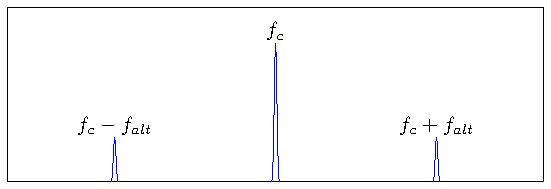
\includegraphics[scale=.95]{../fase/Data/am_details_a.pdf}
  \caption{Sinusoidal carrier modulated by a sinusoidal signal.}
  \label{am_details_a}
\end{figure}

Figure~\ref{am_details_a} shows the spectrum of an ideal carrier signal (at frequency $f_c$) that is modulated by an ideal sinusoidal signal at frequency $f_{alt}$. In addition to the carrier signal, this spectrum has strong ``side-band'' signals offset by $f_{alt}$, i.e. at frequencies $f_c - f_{alt}$ and $f_c + f_{alt}$. This would be the spectral pattern to look for when a periodic signal has a perfectly stable frequency and is modulated by a pattern of activity with a fixed period of $T_{alt} = 1/f_{alt}$ with no variation in timing but these ideal conditions are rarely present in unintentional signals.

\begin{figure}[thb]
  \centering
    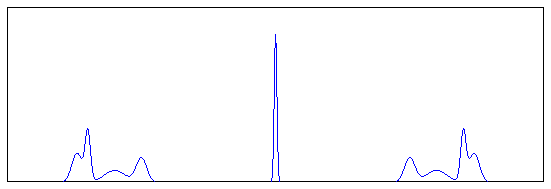
\includegraphics[scale=.95]{../fase/Data/am_details_b.pdf}
  \caption{Sinusoidal carrier modulated by an arbitrary signal.}
  \label{am_details_b}
\end{figure}

Figure~\ref{am_details_b} shows the spectrum of an ideal sinusoidal carrier modulated by an realistic baseband signal. The two side-band signals now correspond to the spectrum of the modulating activity. The tallest spike in each side-band signal corresponds to the dominant periodic behavior of that activity and the smaller ``bumps'' in each side-band signal indicate other common periods of repetitive activity. 

\begin{figure}[h]
  \centering
    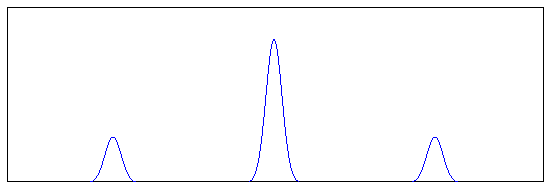
\includegraphics[scale=.95]{../fase/Data/am_details_c.pdf}
  \caption{Non-ideal carrier modulated by a sinusoidal signal.}
  \label{am_details_c}
\end{figure}

Figure~\ref{am_details_c} shows a non-ideal carrier modulated by an ideal signal. The spectrum for the carrier is now spread around its nominal value and this spreading is also present in the two side-band signals. Even though the $f_{alt}$ sinusoid is perfectly stable, the side-bands at $f_c - f_{alt}$ and $f_c + f_{alt}$ will ``inherit'' the instability of $f_c$. Many periodic signals are spread out in this manner in computer systems. For example, spread-spectrum clocking results in deliberate spreading of the clock signal's frequency. Additionally, many periodic activities (e.g. voltage regulator switching) do not require precise timing, so they often use less stable (cheaper/simpler) oscillators. Combining a non-ideal carrier (Figure~\ref{am_details_c}) with a non-ideal modulating activity (Figure~\ref{am_details_b}) produces the spectrum in Figure~\ref{am_details_d}. These non-idealities are typical for program-generated repetitive behavior: for a given task, the time each repetition of the task takes is not always the same, but there are often several commonly-occurring execution times among the repetitions. For example, in multi-processor or SMT systems the repetitions of a loop may take longer or shorter depending on timing variations due to resource contention with other running threads. 

\begin{figure}[thb]
  \centering
    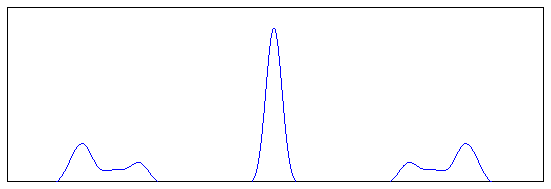
\includegraphics[scale=.95]{../fase/Data/am_details_d.pdf}
  \caption{Non-ideal carrier modulated by an arbitrary signal.}
  \label{am_details_d}
\end{figure}

\section{EM Side Channel Information Leakage on Complex Devices}

Research interest in EM side channel attacks on processors increased with the adoption of smartcards (\eg EMV ``chip'' credit/debit cards). Smartcards have processors operating at speeds less than 30 MHz and usually execute a single cryptographic program. EM emanations resulting from this program activity can leak information about embedded cryptographic keys~\cite{Rao02, Olivier01}. These processors have extremely simple architecture and micro-architecture such as 8-bit and 16-bit data widths, no branch prediction, no data or instruction caches, and small on-chip RAM with deterministic single cycle memory access times.

Despite the ubiquity of cryptographic applications in servers, desktops, laptops, and smartphones there are relatively few published applications of EM emanations targeting complex computing devices such as multi-core, multi-threaded processors with out-of-order execution and external memory interfaces. Attacking such devices is difficult because performance optimizations make emanations more difficult to analyze and because many side-channel attacks require capturing signals at a sampling rate much faster than device's clock rate, which is impractical for GHz clocks~\cite{genkin_2014}. Despite these difficulties, it has been shown that information can be transmitted several meters by EM emanations~\cite{Durak1999}, even in the presence of significant countermeasures (metal shielding, walls, etc.)~\cite{Zajic14}, and cryptographic keys can be extracted from modern computers using EM side-channel analysis~\cite{genkin_2014}. From an EMC perspective, these more powerful systems require more sophisticated components (such as processor and external DRAM memory), larger currents, longer wires, and higher switching frequencies, which all create stronger EM emanations. Therefore the information leakage in these systems may be significant yet difficult to measure and analyze.
%cite something

\section{Emerging EM Emanations Applications Beyond Side Channel Attacks}

Recent work has proposed using side channel EM emanations for several new applications such as disassembling a running program based on EM emanations alone~\cite{eisenbarth2010, scandalee}, instruction profiling for security~\cite{msgna2014}, and also verifying control flow to detect the insertion of malware or other intrusions~\cite{msgna2014_verifying,becker2012,msgna2013}. These existing approaches typically focus on identifying individual instructions (which does not work on complex devices for reasons described in Section~\ref{sec:id_quant_em}) and do not address predicting control flow through entire realistic programs. 

Several other works have shown that some system behaviors in complex devices can be recognized on long timescales. For example, web pages loaded by a device can be distinguished~\cite{Crampton2013}, and malware can be detected~\cite{clark2013} by observing current fluctuations in a power outlet. These approaches treat the leakage mechanism connecting the desired information about the system to the EM emanations as a black box, similar to cryptographic side channel attacks such as DPA. Extracting complex and abstract information about program behavior is difficult with this black box approach. For example, the control flow through a program can be determined or verified by determining whether each branch encountered is taken or not taken. This in itself requires detailed analysis and knowledge of the structure of the program being analyzed, and this structure is different for every different program analyzed. Furthermore, in order to determine the path taken we also need to determine the \textit{time} at which each branch occurs which requires further knowledge of the time required to execute each basic block in the program. 

\section{Traditional Program Profiling}

Program profiling information is used for code optimization (\eg \cite{Debray:2002:PCC:512529.512542}), testing and debugging (\eg \cite{Chilimbi:2009:HES:1555001.1555020}), and software maintenance (\eg \cite{Ernst:1999:DDL:302405.302467}). Unfortunately, obtaining code profiles, and in particular path profiles, requires code instrumentation, which is invasive and comes at the cost of high runtime overhead. The path profiling algorithm proposed by Ball and Larus~\cite{Ball:1996:EPP:243846.243857}, for instance, is an efficient (acyclic) path profiling technique that forms the basis of many other path profilers. This technique was reported to impose an average runtime overhead of 50\%, with as much as a 132\% overhead in the worst case.  Other studies (\eg
\cite{Bond:2005:PPP:1048922.1048988,Vaswani:2007:PPP:1190216.1190268}) also report similarly high overhead.

A number of techniques have been proposed by researchers to reduce the overhead of profiling. Many of these approaches try to extend or modify Ball and Larus's technique. Selective path profiling techniques (\eg \cite{Vaswani:2007:PPP:1190216.1190268,Bond:2005:PPP:1048922.1048988,Apiwattanapong:2002:SPP:586094.586104, ProfilingSelectedPathsWithLoops}) aim to reduce the overhead of path profiling by selecting a given set of paths, based on the observation that only a subset of program paths are normally of interest. Targeted path profiling~\cite{Joshi:2004:TPP:977395.977660} is another related approach that tries to reduce the execution overhead by not instrumenting the regions in the code where information could be obtained using edge profiling. Pertinent path profiling~\cite{Baswana:2013:PPP:2495258.2495922} is yet another technique that addresses the high overhead problem by optimizing the data structures used for profiling. Sampling-based instrumentation approaches (\eg ~\cite{Arnold:2001:FRC:378795.378832,  Traub00ephemeralinstrumentation}) use a different approach to reduce the cost of instrumentation and infer profiling information from a sample of runtime events. Finally, partitioned path profiling~\cite{Afraz:2015:PPP:2786805.2786868} proposes the idea of parallel path profiling, which profiles a program by evenly distributing the number of probes into multiple cores.

Despite all the work done so far to reduce the runtime overhead of instrumentation based program profiling, profiling still comes at a non-negligible cost in terms of overhead. Although this overhead is tolerable in some cases, it is not always so (\eg for embedded devices with limited resources or real-time systems). Moreover, instrumentation is an intrusive technique that can change some aspect of a program's dynamic behavior of such code, especially in the case of complex, real-time, and/or multi-threaded systems. %This system has zero overhead while profiling executions. In return for zero overhead, ZOP requires a training phase and the accuracy is imperfect. This reduction in accuracy may be acceptable for many applications.

Some systems have hardware features to assist in profiling~\cite{intel_vtune, intel_pmu, arm_pmu, shye2005}, but these features cannot completely eliminate software overhead; even hardware-accelerated profiling must somehow record profiling information, which necessarily affects the programs being profiled. External hardware tracers and debuggers~\cite{lauterbach} can profile without software overhead but require significant processor hardware support to collect and transmit traces off-chip. Using EM emanations, profiling has no in-system hardware requirements, which is particularly appealing for applications where any overhead, instrumentation, or modification is unacceptable and for systems where hardware profiling support is unavailable.
